\section{The Structure of \jel{} System}
\label{sec:The_Components_of_the_Jeliot_3_System}

We introduce here the different components of \jel{} systems. The system
contains several packages and here we explain those that are most crucial
in understanding the structure of \jel{}. Only package and classes related
to communication between visualization engine and \djava{} are introduced
in the chapter~\ref{sec:Communications_Model}.

The functional structure of the Jeliot~3 is shown in the
Figure~\ref{fig:structure_of_jeliot_3}. A user interacts with the user
interface and forms the source code of the program (1). The source code
is sent to the Java interpreter and the intermediate code is extracted
(2 and 3). The intermediate code is interpreted and the directions are
given to the visualization engine (4 and 5). A user can control the
animation by playing, pausing, rewinding or playing step-by-step the
animation through the user interface (6). Furthermore, the user can
input data, for example, an integer or a string, to the program
executed by the interpreter (6, 7 and 8).

\begin{figure}[htbp]
\begin{center}
\begin{picture}(400,250)

% BOXES, OVALS and CIRCLE
%--------------------------
%User group
\put(50,30){\circle{60}}
\put(20,0){\makebox(60,60){\f{User}}}
%User interface
\put(10,90){\framebox(80,20){\f{User interface}}}
%Source code
\put(50,200){\oval(80,50)}
\put(10,175){\makebox(80,50){\shortstack{\f{Source code}\\\f{of the program}}}}
%DJava
\put(160,160){\framebox(80,80){\shortstack{\f{Interpretation}\\\f{of the program}\\\f{code done by}\\\f{\djava{}}}}}
%Intermediate code
\put(350,200){\oval(80,70)}
\put(310,165){\makebox(80,70){\shortstack{\f{Intermediate}\\\f{code of the}\\\f{program}\\\f{execution}}}}
%Visualization engine
\put(160,60){\framebox(80,50){\shortstack{\f{Visualization}\\\f{engine}}}}
%Intermediate code Interpreter
\put(310,60){\framebox(80,50){\shortstack{\f{Intermediate}\\\f{code}\\\f{Interpreter}}}}
% VECTORS
%----------------------------
% 0. (user, user interface) (user interface, user)
\put(40,47){\vector(0,1){43}}
\put(60,90){\vector(0,-1){43}}
% 1. (user interface, source code)
\put(50,110){\vector(0,1){65}}
\put(50,110){\makebox(20,65){\f{1.}}}
% 2. (source code, djava)
\put(90,200){\vector(1,0){70}}
\put(90,200){\makebox(70,20){\f{2.}}}
% 3. (djava, intemediate code)
\put(240,200){\vector(1,0){70}}
\put(240,200){\makebox(70,20){\f{3.}}}
% 4. (intemediate code, intemediate code interpreter)
\put(350,165){\vector(0,-1){55}}
\put(350,110){\makebox(20,55){\f{4.}}}
% 5. (intemediate code interpreter, visualization engine)
\put(310,100){\vector(-1,0){70}}
\put(240,100){\makebox(70,20){\f{5.}}}
% 6. (user interface, visualization engine)
\put(90,100){\vector(1,0){70}}
\put(90,100){\makebox(70,20){\f{6.}}}
% 7. (intemediate code interpreter, visualization engine)
\put(240,80){\vector(1,0){70}}
\put(240,80){\makebox(70,20){\f{7.}}}
% 8. (visualization engine, Djava)
\put(310,110){\vector(-1,1){70}}
\put(260,130){\makebox(50,50){\f{8.}}}
\end{picture}
\caption{The functional structure of Jeliot~3.}
\label{fig:structure_of_jeliot_3}
\end{center}
\end{figure}

Different packages of \jel{}~3 are introduced in this section in
the same order as in the functional structure. In this way we
hope that all the components and their meaning becomes clearer.

\subsection{\jel{} Class}
\label{sec:Jeliot_Class}

Class \jel{} in the package \p{jeliot} is the main class of the program.
It combines the different components of the program together a deals with
some communicational issues. When the program is started the class creates
all the needed components and passes them as parameters to the user interface
classes. It mainly handles the communication between the user interface
(\p{jeliot.gui}) and the theater/animation engine (\p{jeliot.theatre}) classes.
In addition to that it also invokes the thread handling the interpretation
of the user program.

\subsection{User Interface}
\label{sec:User_Interface}

The user interface of Jeliot is located in the package \p{jeliot.gui}.
The structure of the user interface is shown in the
Figure~\ref{fig:jeliot3_UI_structure}. The main
class is \p{JeliotWindow} that extends \p{JFrame}. The frame is layed out
by \p{BorderLayout}. A split pane (\p{JSplitPane}) is added in the center and
a panel containing control panel (created in \p{JeliotWindow}) and output console
(\p{OutputConsole}) is added in the south (bottom) border.

In the split pane the left side is used by code editor (\p{CodeEditor}) or code viewer
(\p{CodeViewer}). Code editor is shown during editing of the program
and code viewer during the animation of the program. Both of the text components
have a line numbering component (\p{LineNumbers} on their row header. Moreover,
code editor consist of editing panel that has a few buttons to load, save and
edit the source code. The frame has also a menu bar that is constructed
partially in \p{CodeEditor} class and partilly in \p{JeliotWindow} class.

On the right hand side of the split pane a animation engine called
theater (\p{Theatre}) is normally shown. However, if any errors occur
during the compilation or run-time of the program they are shown
in the \p{Error viewer} (\p{ErrorViewer}) instead of theater.

\p{JeliotWindow} combines all the components in \p{jeliot.gui} package and
creates the user interface. It also deals with most of the events
happening during the {run-time} and delegates the commands forward to
the appropriate classes (e.g. \p{Jeliot} or \p{CodeEditor}). Other classes
in the \p{gui} package are related to one of the components introduced in the
previous paragraph. There are also three classes that are not currently in use
in \jel{}~3, namely \p{LoadJeliot}, \p{DraggableComponent} and \p{TheatrePopup}.

\begin{figure}[htbp]
\begin{center}
\begin{picture}(300,200)
%overall frame
\put(0,0){\framebox(300,200){\ }}
%Menu bar
\put(0,170){\framebox(100,30){\f{Menu bar}}}
%Code editor
\put(0,40){\framebox(100,130){\shortstack{\f{Code editor}\\\f{or}\\\f{Code viewer}}}}
%Theatre
\put(100,40){\framebox(200,160){\shortstack{\f{Animation frame (Theatre)}\\\f{or}\\\f{Error viewer}}}}
%Control panel
\put(0,0){\framebox(120,40){\f{Control panel}}}
%Output Console
\put(120,0){\framebox(180,40){\f{Output Console}}}
\end{picture}
\caption{The structure of user interface in Jeliot~3.}
\label{fig:jeliot3_UI_structure}
\end{center}
\end{figure}

\subsection{DynamicJava}
\label{sec:DynamicJava}

DynamicJava consists of 7 different packages, where only five
of them actually perform the interpretation: \p{classfile}, \p{classinfo},
\p{interpreter}, \p{parser} and \p{tree}. The other two (\p{util} and \p{gui}) are
used to help the debugging of DynamicJava and to provide a nicer
user interface to the interpreter. For example, the \p{displayVisitor},
included in the util package, provides a nice output from the syntax tree.

\begin{itemize}
\item \p{Classfile} contains all the classes for creating general purpose bytecode
classes. The most important class is ClassFile which is the heart
of the class creation process.

\item \p{Classinfo} contains all the classes and interfaces for using reflection
on Java or interpreted classes. This package is used during
the compilation of the classes.

\item \p{Interpreter} contains the classes for interpreting Java language statements.
This is the most important package. It contains the most important
visitors that will be explained later.

\item \p{Parser} provides the classes that compose the default parser for the
language. The parser itself is represented by the class \p{Parser}.
The parser is generated by JavaCC 1.0. It creates the nodes of the
tree to be traversed later by the interpreter visitors.

\item \p{Tree} provides classes and interfaces for producing an abstract syntax
tree. This package does not depend of any non standard java package.

The created tree consists of nodes, the main data structure used
in \djava{}. All nodes have common properties, the segment
of source code where that node refers. Subclasses of this node
are defined to address the unique properties of each different
Java (e.g. staments and constructions). For example a node for
any binary expression will also consist of the properties \p{LEFT\_EXRESSION}
and \p{RIGHT\_EXPRESSION}.

\end{itemize}

Figure \ref{fig:Packages_visitors_and_data_flow_in_DJava} explains the
main relationships between the packages, the visitors and the main data flow.

\begin{figure}[htbp]
\begin{center}
\begin{picture}(400,200)
\put(110,20){\framebox(270,130){\ }}
\put(220,20){\makebox(50,20){\f{Interpreter}}}

\put(0,50){
\put(0,15){\vector(1,0){40}}
\put(0,15){\makebox(40,20){\shortstack{\f{source}\\\f{code}}}}
\put(40,0){\framebox(50,30){\f{Parser}}}
\put(90,15){\vector(1,0){40}}
\put(90,15){\makebox(40,20){\f{tree}}}
\put(130,0){\dashbox{5}(55,30){\shortstack{\f{Name}\\\f{Visitor}}}}
\put(185,15){\vector(1,0){35}}
\put(180,15){\makebox(40,20){\f{tree}}}
\put(220,0){\dashbox{5}(55,30){\shortstack{\f{Type}\\\f{Checker}}}}
\put(275,15){\vector(1,0){35}}
\put(270,5){\makebox(40,20){\shortstack{\f{tree}\\\f{and}\\\f{class}}}}
\put(310,0){\dashbox{5}(55,30){\shortstack{\f{Evaluation}\\\f{Visitor}}}}
\put(365,15){\vector(1,0){35}}
\put(360,15){\makebox(40,20){\f{result}}}
}

\put(240,80){\vector(0,1){20}}\put(250,100){\vector(0,-1){20}}
\put(240,130){\vector(0,1){40}}\put(250,170){\vector(0,-1){40}}
\put(60,80){\vector(0,1){90}}\put(70,170){\vector(0,-1){90}}
\put(270,180){\vector(1,0){40}}\put(310,190){\vector(-1,0){40}}

\put(220,100){\dashbox{5}(55,30){\shortstack{\f{TreeClass-}\\\f{Compiler}}}}

\put(0,170){
\put(40,0){\framebox(50,30){{\f{Tree}}}}
\put(220,0){\framebox(50,30){{\f{ClassInfo}}}}
\put(310,0){\framebox(50,30){{\f{ClassFile}}}}
}

\end{picture}
\caption{Packages, visitors and data flow in \djava{}}
\label{fig:Packages_visitors_and_data_flow_in_DJava}
\end{center}
\end{figure}

As we can see in the image DynamicJava carries the source code
through three visitors: \p{NameVisitor}, \p{TypeChecker} and, finally,
\p{EvaluationVisitor}. We also see how \p{EvaluationVisitor} will receive
a class from \p{TypeChecker}, the reason of this behaviour will be explained
in the next paragraphs.

The NameVisitor is a tree visitor that resolves the ambiguity in identifiers
in a syntax tree. As declared, this visitor traverses the tree trying to find
out syntactical ambiguities.

The \p{TypeChecker} is a tree visitor that checks the typing rules and loads the
classes, fields and methods. This \p{TypeChecker} class is not only worried
about typing rules. When visiting a class declaration, it invokes
\p{TreeCompiler}, which compiles the class into Java bytecode. However, this
compiling process \textit{alters the class} and the formed \textit{bytecode
does not match the original source code} of the class.

The \p{EvaluationVisitor} is a tree visitor that evaluates each node of
a syntax tree. This visitor is the one that performs the evaluation and
execution of the program. It usually starts by invoking the main method
of the compiled class. We can easily observe how it traverses
the syntax tree and modifies \djava{} structures to store information
and thus we can interfere with its normal interpretation to extract
the information it produces while interpreting the source code.

\subsubsection{Tree package}
\label{sec:Tree_package}

See the Figures~\ref{fig:several_tree_classes},
\ref{fig:primary_expression_classes}, \ref{fig:statement_classes},
\ref{fig:un_and_bin_exp_classes}.

\begin{figure}[!htb]
\begin{center}
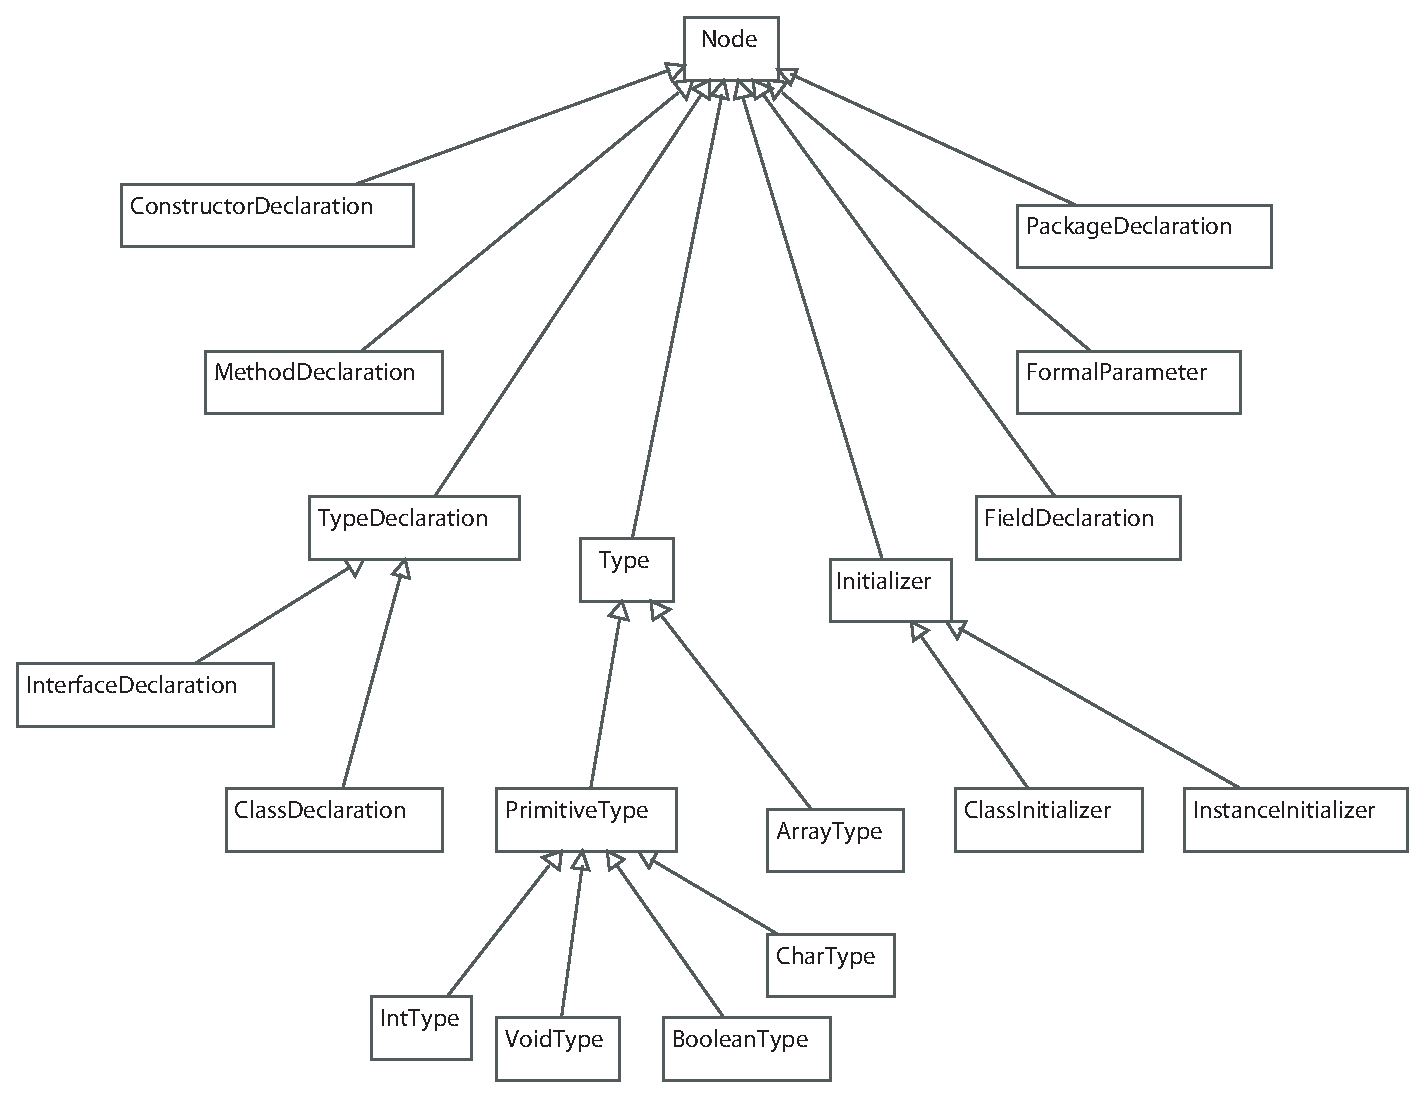
\includegraphics[width=\textwidth]{images/several.eps}
\caption{Several Tree classes. (Change the caption)}
\label{fig:several_tree_classes}
\end{center}
\end{figure}

\begin{figure}[!htb]
\begin{center}
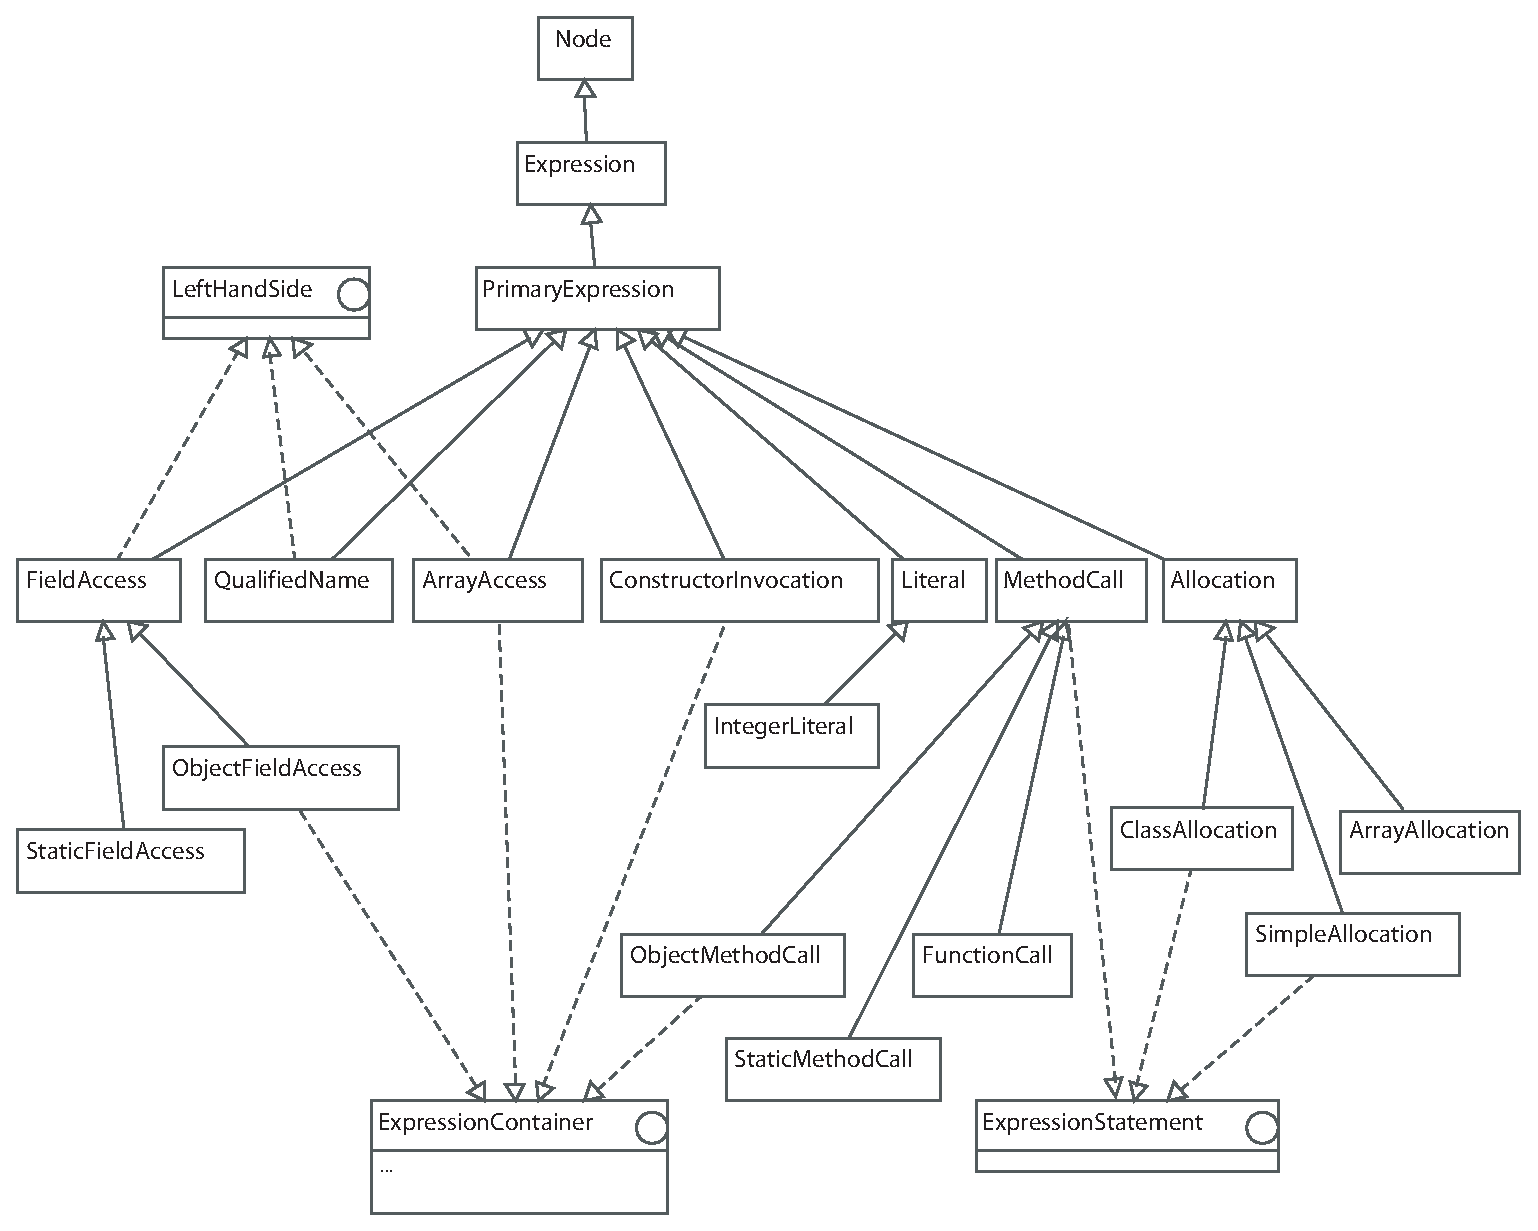
\includegraphics[width=\textwidth]{images/primaryexpressions.eps}
\caption{Primary expressions classes in \p{tree} package. (Change the caption)}
\label{fig:primary_expression_classes}
\end{center}
\end{figure}

\begin{figure}[!htb]
\begin{center}
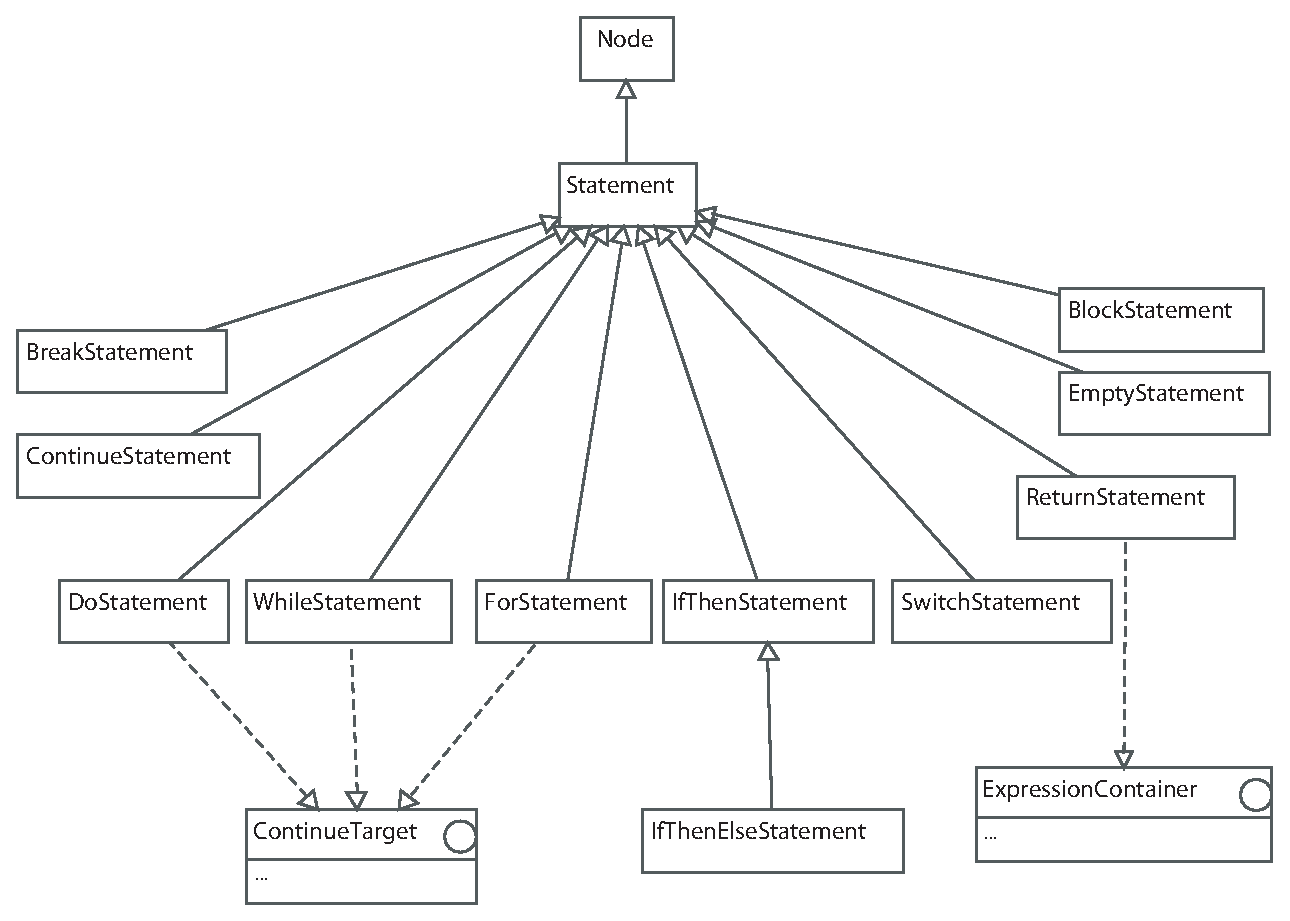
\includegraphics[width=\textwidth]{images/statements.eps}
\caption{Statement classes in \p{tree} package. (Change the caption)}
\label{fig:statement_classes}
\end{center}
\end{figure}

\begin{figure}[!htb]
\begin{center}
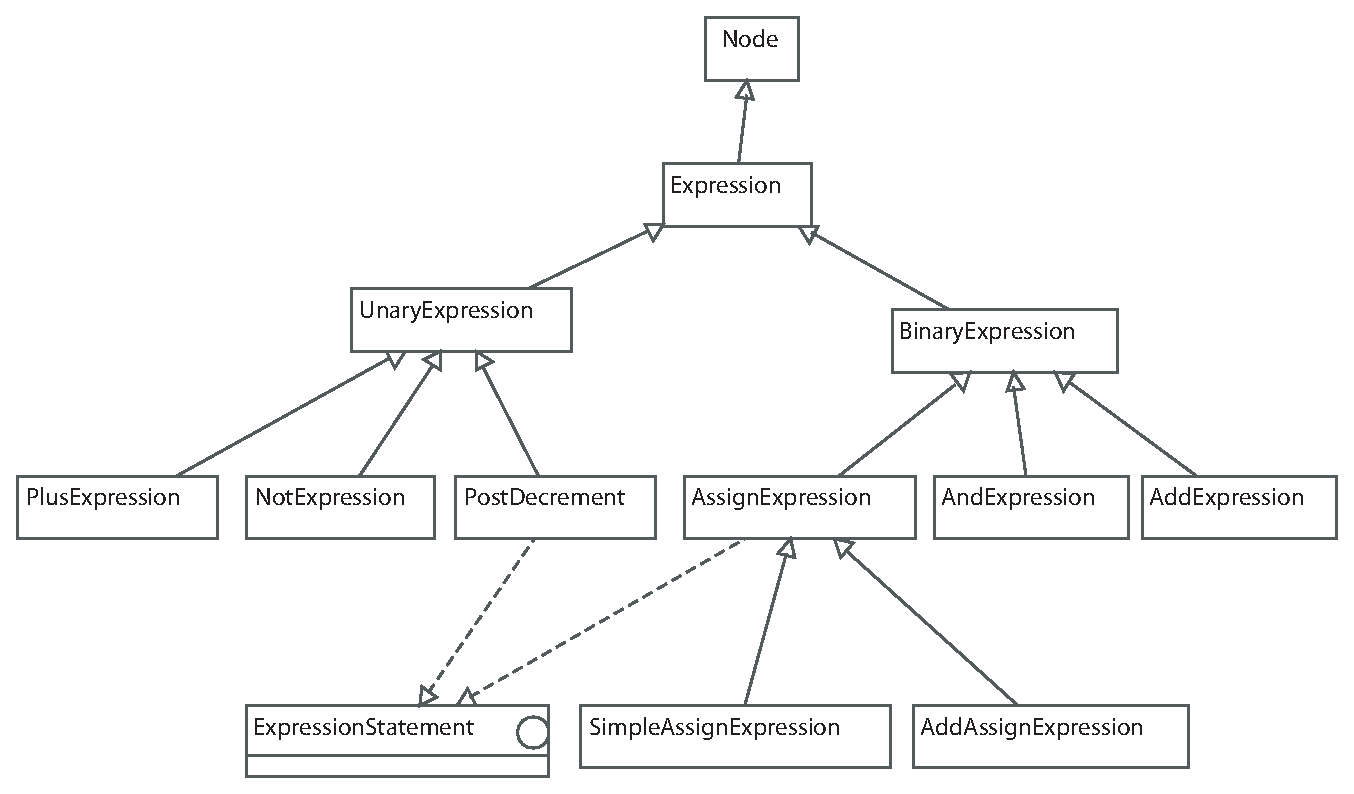
\includegraphics[width=\textwidth]{images/unary-bin-exps.eps}
\caption{Unary and binary expression classes in \p{tree} package. (Change the caption)}
\label{fig:un_and_bin_exp_classes}
\end{center}
\end{figure}

\subsection{Intermediate Code Interpreter}
\label{sec:Intermediate_Code_Interpreter}

The package \p{jeliot.ecode} includes the classes used by the intermediate
code interpreter. The class \p{Interpreter} contains the intermediate code
interpreter and the other classes  help the work with intermediate
code generation, interpretation and on the other aspects of the program execution.

The intermediate code is generated by the modified version of \djava{}. The code is
then written into a pipe that can be read by the interpreter. As the code is completely
machine written we know the form of the code and can interpret it easily. The intermediate
code is introduced in the section~\ref{sec:Intermediate_Code}. The code is read
line by line and it is tokenized with the agreed token in the class \p{Code} that contains
all the necessary constants for intermediate code generation. Then the first token tells what kind of statement is coming and how it should be processed. Then the rest of the statement is processed accordingly and a part of the animation is shown if necessary.

There are several data structures in the \p{Code} class.
\begin{description}
\item[\p{commands}] variable is a reference to a hash table that contains information about each given command. Command in this context tells, for instance, whether a operand of a binary operation is the left or right side of the operation.
\item[\p{exprs}] variable is a reference to a hash table containing the information about each expression. The information consist of each expressions type (e.g. addition or subtraction operation), expression reference and the location in the code.
\item[\p{values}]
\item[\p{variables}]
\item[\p{instances}]
\item[\p{methodInvocation}]
\item[\p{postIncsDecs}]
\item[\p{currentClass}]
\item[\p{classes}]
\item[\p{currentMethodInvocation}] 
\item[\p{objectCreation}]
\item[\p{returned, returnValue, returnActor, returnExpressionCounter}] are variables for handling the return value of a method.
\end{description}

Class \p{ECodeUtilities} is used by the interpreter to help type identification and
translating the intermediate code into the commands used in the visualization engine because they differ in some parts. It also handles some issues related to user input
and communication between \djava{} and the intermediate code interpreter. 

\subsection{Language Constructs}
\label{sec:Language_package}

The classes of \p{jeliot.lang} package represent Java language constructs.

See Figure~\ref{fig:language_constructs_and_actors}.

\begin{figure}[!htb]
\begin{center}
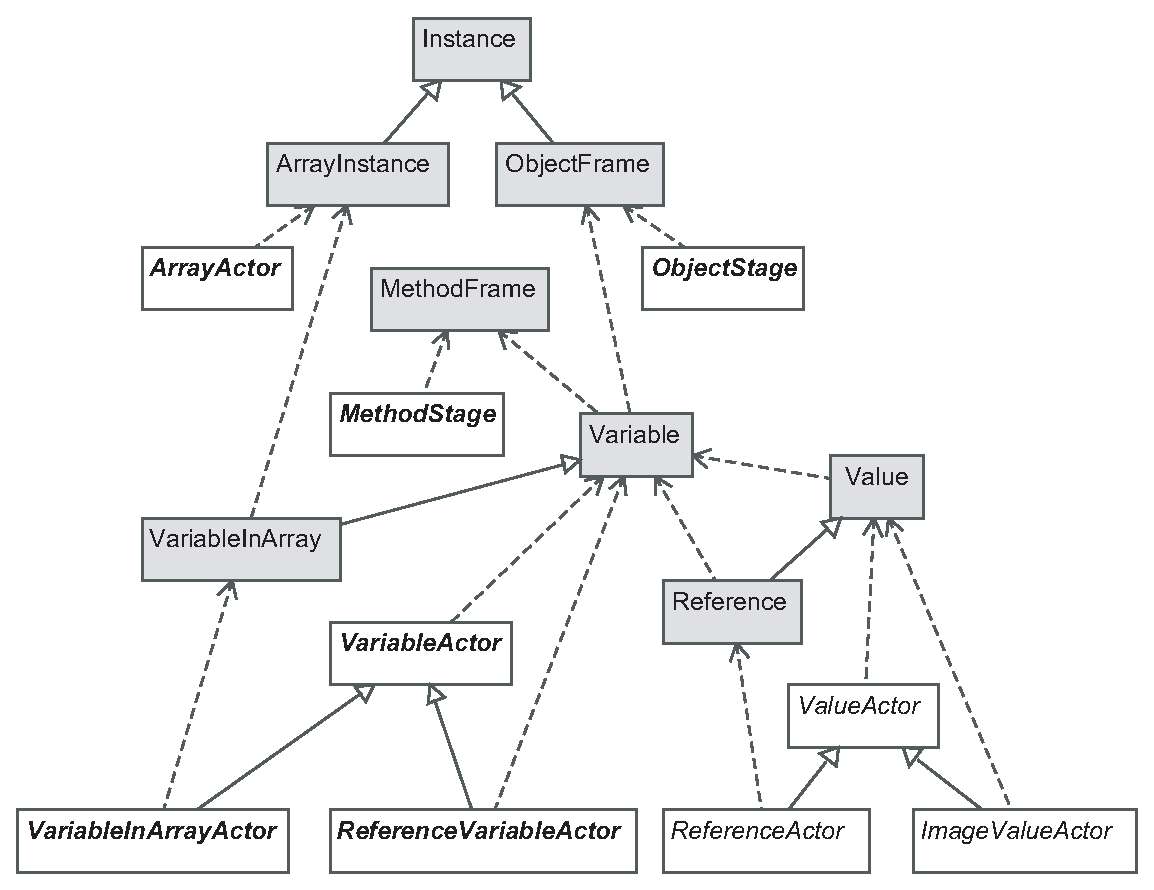
\includegraphics[width=\textwidth]{images/language_constructs_and_actors.eps}
\caption{The class hierarchy of the language constructs (gray boxes and solid lines) and the \p{Actor}s (white boxes and solid lines) and their usage relations to each other (dashed lines). \p{Actor}s (white boxes) implementing actor container are written in bold and italics and the other \p{Actor}s on just italics.}
\label{fig:language_constructs_and_actors}
\end{center}
\end{figure}

\subsection{Visualization Engine}
\label{sec:Visualization_Engine}

The package \p{jeliot.theatre} contains classes that are used by the animation
component called \p{Theatre}. We will here introduce the most important
classes in the package and tell the meaning of these classes. For rest of
the class see the documented source code.

See Figure~\ref{fig:jeliot3_theatre_structure}.

\begin{figure}[htbp]
\begin{center}
\begin{picture}(250,200)
%Overall frame
\put(0,0){\framebox(250,200){{\f{\bf{Theatre}}}}}
%Method frame area
\put(10,100){\dashbox{5}(80,90){\shortstack{\f{Method}\\\f{Stage}\\\f{Area}}}}
%Constant box
\put(10,10){\dashbox{5}(60,30){\shortstack{\f{Constant}\\\f{Box}}}}
%Instance Area
\put(80,10){\dashbox{5}(160,80){\shortstack{\f{Instance}\\\f{Area}}}}
%Expression Evaluation Area
\put(100,110){\dashbox{5}(140,80){\shortstack{\f{Expression}\\\f{Evaluation}\\\f{Area}\\\f{(Scratch)}}}}
\end{picture}
\caption{The structure of the animation frame (theatre) in Jeliot~3.}
\label{fig:jeliot3_theatre_structure}
\end{center}
\end{figure}

\subsubsection{Director class}

\p{Director} has a methods for different kind of operations during the
animation of the program (e.g. binary expression, unary expression,
object creation and method call). These methods are called by the intermediate code
interpreter (\p{ECodeInterpreter}). In each of the methods are given parameters
that the method needs for the operation.

Normally, first the method creates actors through \p{ActorFactory}
or uses existing actors. \p{Animation}s are created through \p{Actor}s' methods
(e.g. \p{appear} or \p{fly}). Created animations are given to
\p{AnimationEngine} to be run.Actors can be also added to other
\p{ActorContainer}s (e.g. \p{Theatre}, \p{VariableActor} or
\p{MethodStage}).

\subsubsection{Actor classes}

See Figure~\ref{fig:class_hierarchy_of_Actor_class_small}.

\begin{figure}[!htb]
\begin{center}
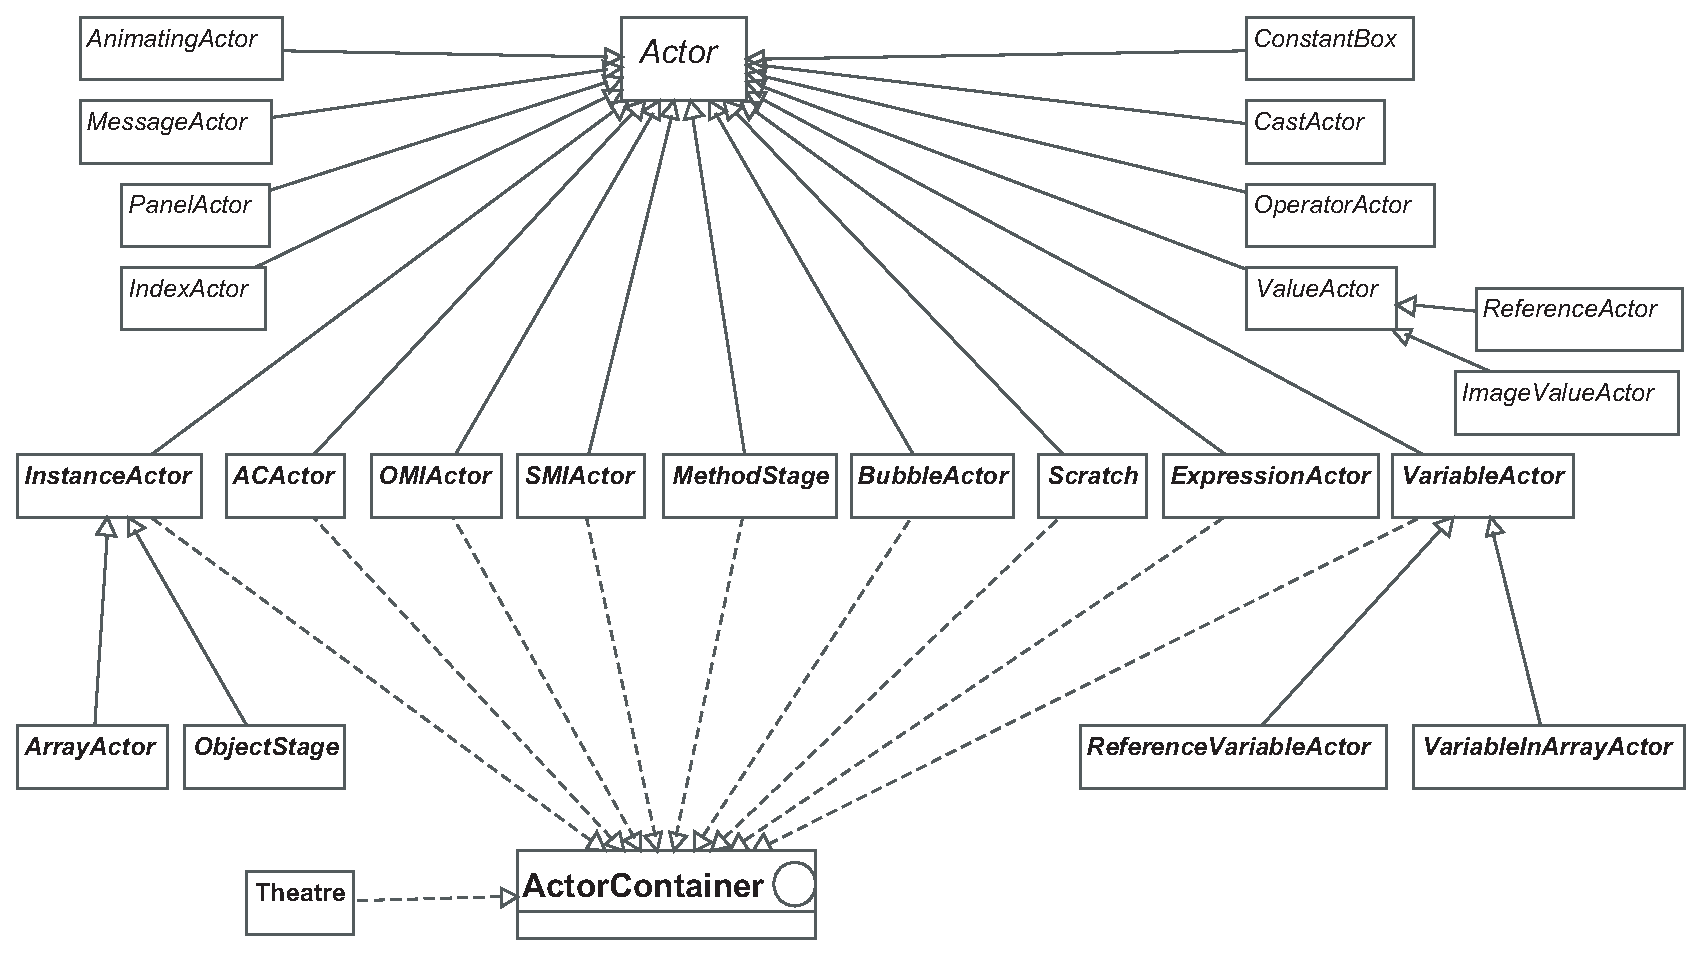
\includegraphics[width=\textwidth]{images/jeliot_actor_class_small.eps}
\caption{The class hierarchy of \p{Actor} class and \p{ActorContainer} interface.}
\label{fig:class_hierarchy_of_Actor_class_small}
\end{center}
\end{figure}

\subsubsection{ActorContainer interface}

See the Figure~\ref{fig:actors_and_actorcontainers}.

\begin{figure}[!htb]
\begin{center}
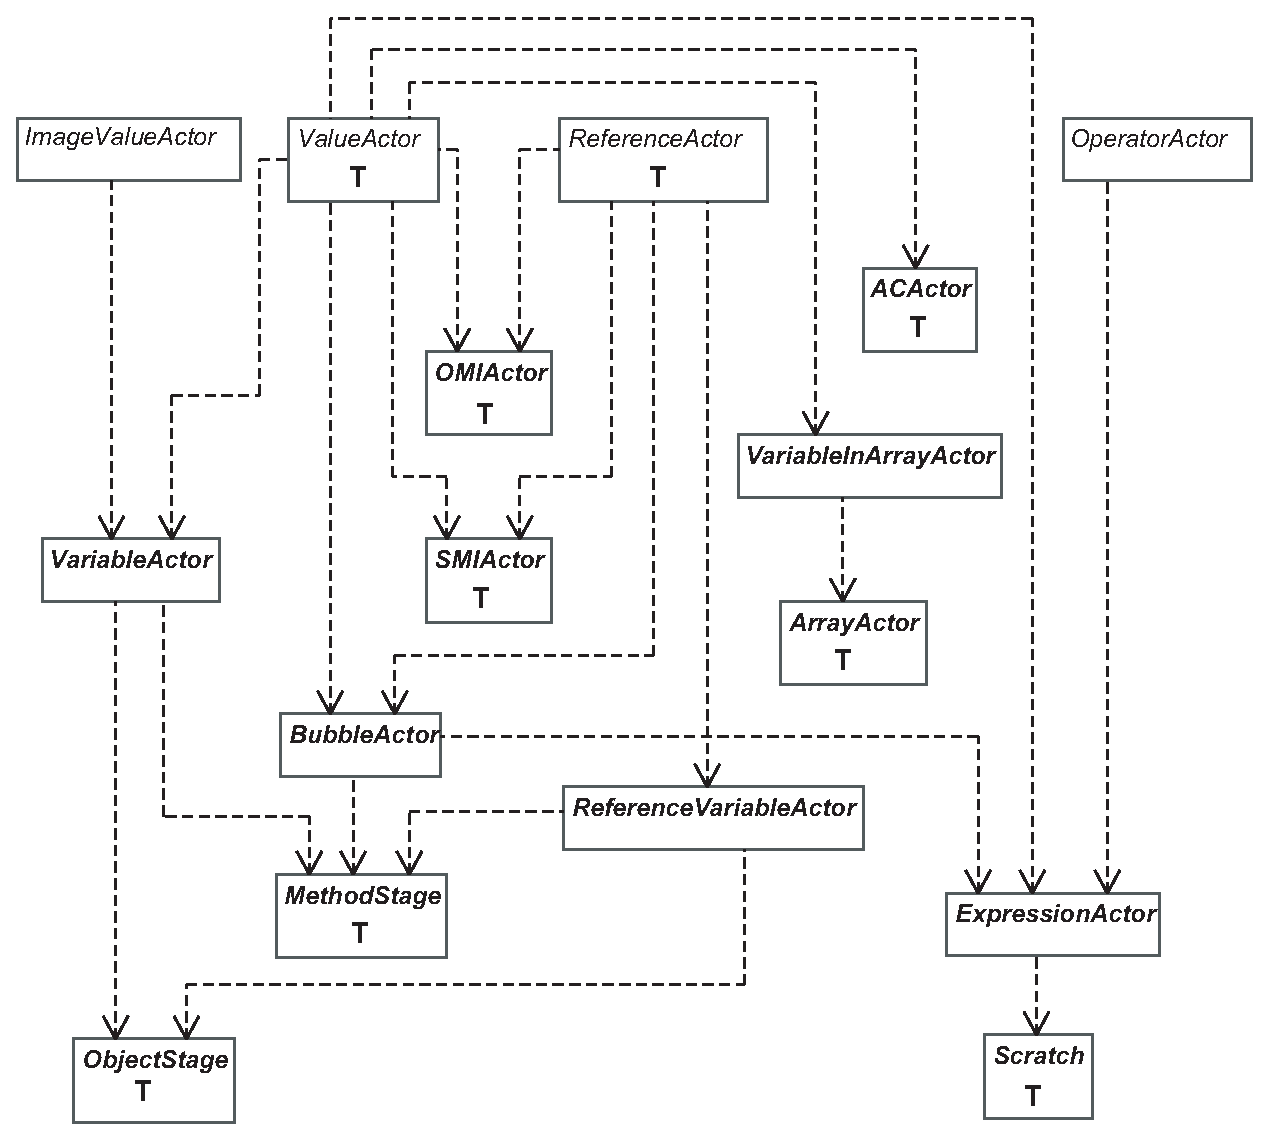
\includegraphics[width=10cm]{images/actorcontainers_and_actors.eps}
\caption{The inclusion relations between \p{Actor}s and \p{Actor}s implementing \p{ActorContainer} interface.}
\label{fig:actors_and_actorcontainers}
\end{center}
\end{figure}

\subsubsection{Animation class}

See the Figure~\ref{fig:jeliot3_animation_engine}.

\subsubsection{AnimationEngine class}

See the Figure~\ref{fig:jeliot3_animation_engine}.

\subsubsection{Theatre class}

See the Figure~\ref{fig:theatre_and_actorcontainers}.

\begin{figure}[!htb]
\begin{center}
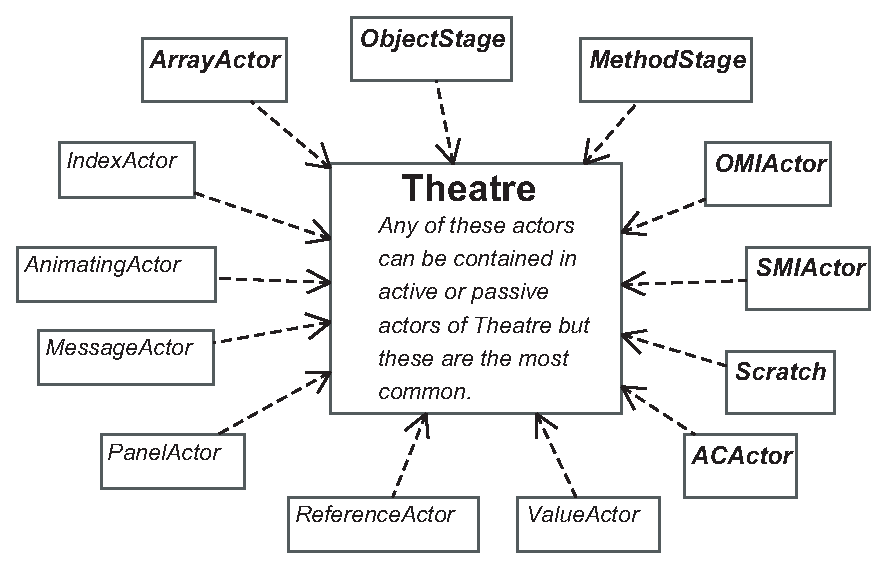
\includegraphics[width=10cm]{images/theatre_and_actors.eps}
\caption{The \p{Actor}s that are commonly included in the passive (\p{pasAct}) and active (\p{actAct}) \p{Actor}s.}
\label{fig:theatre_and_actorcontainers}
\end{center}
\end{figure}


\begin{figure}[!htb]
\begin{center}
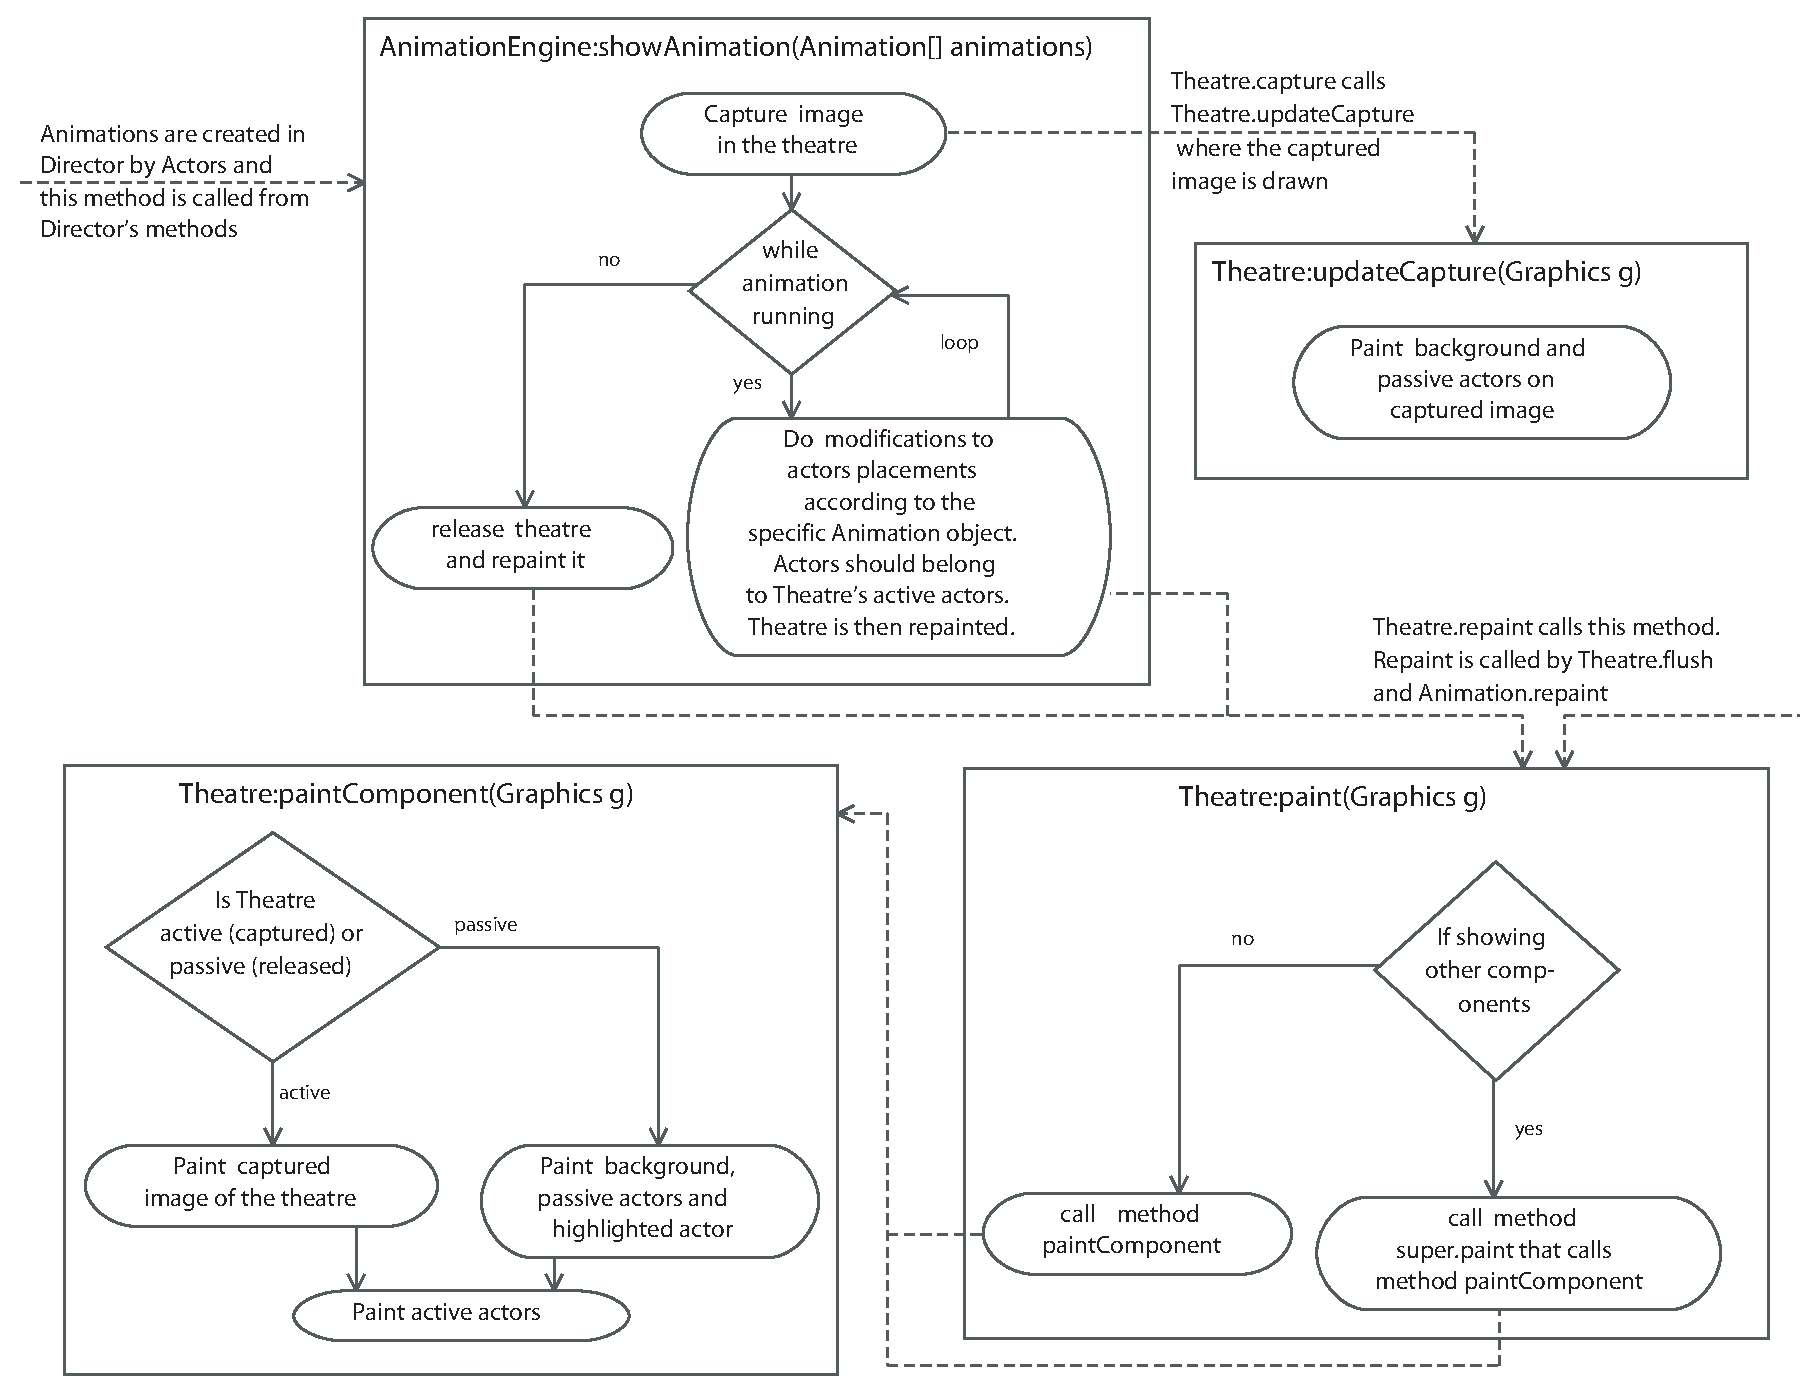
\includegraphics[width=\textwidth]{images/jeliot_animation_engine3.eps}
\caption{The structure of the animation engine in \jel{}.}
\label{fig:jeliot3_animation_engine}
\end{center}
\end{figure}

\subsubsection{TheatreManager class}


\subsubsection{ActorFactory class}

